%-----------------------------------------------
% Template para criação de resumos de projectos/dissertação
% jlopes AT fe.up.pt,   Fri Jul  3 11:08:59 2009
%-----------------------------------------------

\documentclass[9pt,a4paper]{extarticle}

%% English version: comment first, uncomment second
\usepackage[portuguese]{babel}  % Portuguese
%\usepackage[english]{babel}     % English
\usepackage{graphicx}           % images .png or .pdf w/ pdflatex OR .eps w/ latex
\usepackage{times}              % use Times type-1 fonts
\usepackage[utf8]{inputenc}     % 8 bits using UTF-8
\usepackage{url}                % URLs
\usepackage{multicol}           % twocolumn, etc
\usepackage{float}              % improve figures & tables floating
\usepackage[tableposition=top]{caption} % captions
%% English version: comment first (maybe)
\usepackage{indentfirst}        % portuguese standard for paragraphs
%\usepackage{parskip}

%% page layout
\usepackage[a4paper,margin=30mm,noheadfoot]{geometry}

%% space between columns
\columnsep 12mm

%% headers & footers
\pagestyle{empty}

%% figure & table caption
\captionsetup{figurename=Fig.,tablename=Tab.,labelsep=endash,font=bf,skip=.5\baselineskip}

%% heading
\makeatletter
\renewcommand*{\@seccntformat}[1]{%
  \csname the#1\endcsname.\quad
}
\makeatother

%% avoid widows and orphans
\clubpenalty=300
\widowpenalty=300

\begin{document}

\title{\vspace*{-8mm}\textbf{\textsc{Journata - Designing the interaction of a mobile application for exchanging public transport information among travellers}}}
\author{\emph{Marco André Moreira Amador}\\[2mm]
\small{Projecto/Dissertação realizado sob a orientação da \emph{Prof.\ Teresa Galvão Dias}}\\}
%\small{na \emph{FazSoft Lda}}}
\date{23 de Junho de 2014}
\maketitle
%no page number 
\thispagestyle{empty}

\vspace*{-4mm}\noindent\rule{\textwidth}{0.4pt}\vspace*{4mm}

\begin{multicols}{2}

\section{Motivação}\label{sec:motiva}

Nos dias que correm, a utilização de dispositivos móveis com acesso à Internet permite o acesso a qualquer momento e em qualquer lugar a uma panóplia de aplicações que permitem aos utilizadores consultar e inclusivamente partilhar diversos tipos de informação em tempo real. 

Neste sentido, foi proposto anteriormente a criação de uma aplicação móvel para partilha de informação sobre transportes públicos em tempo real.

Esta aplicação é bastante inovadora, dado que a origem da informação partilhada são os próprios utilizadores, que partilham entre si vários aspectos da viagem ou condutor. Outra das grandes inovações é a forma como os utilizadores estão ligados entre si, através da criação de redes sociais dinâmicas no tempo e no espaço, centradas no utilizador.

Este trabalho pretende melhorar a interface e interacção da aplicação desenvolvida anteriormente, tornando-a mais atractiva, com vista a melhorar a experiência de utilização das redes de transporte público por parte dos seus utilizadores, numa tentativa de eliminar os tempos de espera ou torná-los mais suportáveis.

\section{Objectivos}\label{sec:goals}

Tendo em conta os aspectos referidos na secção anterior, pretende-se com este trabalho desenvolver uma interface de utilização da referida aplicação, cumprindo os seguintes objectivos:

\begin{itemize}
\item Criar e analisar metáforas adequadas para a interacção com o conceito de redes sociais dinâmicas.
\item Aplicar conceitos 'estado-da-arte' relacionados com Interacção Pessoa-Computador para maximizar a usabilidade da interface desenvolvida, resolvendo também problemas de usabilidade já identificados numa iteração anterior do projecto.
\item Desenvolver um protótipo funcional para uma aplicação móvel \emph{Android} tendo por base protótipos de baixo nível desenvolvidos até então.
\item Testar o sistema e avaliar os resultados obtidos.
\end{itemize}

\section{Descrição do Problema}\label{sec:work}

Tendo em conta que a informação na plataforma é partilhada entre utilizadores da aplicação, a usabilidade da referida aplicação é um aspecto fundamental para o sucesso e adopção da mesma entre os passageiros das redes de transporte público.

Nesse sentido, destaca-se a importância de escolher um processo de desenvolvimento que envolvesse utilizadores finais e \emph{experts} da área de usabilidade na validação e evolução da interface.

Optou-se então por um processo constituído por quatro fases:
\begin{itemize}
\item \textbf{Definição de Requisitos de Usabilidade} - Inclui a análise de limitações na óptica de usabilidade presentes na iteração anterior da aplicação, a criação de soluções de \emph{design} com vista a resolver essas limitações, e a discussão dessas soluções num \emph{focus group} com potenciais utilizadores da aplicação.
\item \textbf{\emph{Design}} - Criação e evolução iterativa de alternativas para a interface da aplicação, com recurso a protótipos de baixo nível.
\item \textbf{\emph{Prototipagem}} - Desenvolvimento de um protótipo funcional para \emph{Android} tendo em conta o obtido na fase anterior.
\item \textbf{\emph{Avaliação}} - Realização de testes e avaliação de usabilidade, e levantamento dos resultados obtidos.
\end{itemize}


\subsection{Definição de Requisitos}\label{sec:req}

A aplicação em questão possuía um conjunto de funcionalidades bem definido, entre as quais se contavam:

\textbf{-} Check-in e checkout num veículo/viagem;

\textbf{-} Consulta de informação sobre o veículo/rota;

\textbf{-} Submissão de comentários.

\textbf{-} Classificação de comentários de outros utilizadores;

\textbf{-} Planeamento de viagem para um futuro próximo.

Após uma análise inicial, concluiu-se que as funcionalidades de check-in e check-out num veículo/rede poderiam estar pouco visíveis para o utilizador, dado o elevado tempo de execução da tarefa revelado em testes feitos anteriormente. De igual modo, a mesma limitação relativa à funcionalidade de classificação de comentários de outros utilizadores foi identificada, relacionada com a dificuldade que os utilizadores tinham em perceber o conceito e a necessidade de fazerem tal coisa.

Foram posteriormente concebidas soluções iniciais de design para vários componentes de navegação e funcionalidades da aplicação que visavam eliminar estas limitações, com o objectivo de as apresentar num \emph{focus group} realizado com potenciais utilizadores, destinado a levantar requisitos de usabilidade para a aplicação.

Essa sessão revelou duas grandes limitações na concepção da aplicação que condicionavam a necessidade de obtenção de informação e os seus hábitos de viagem: impossibilidade de receber informação sobre um veículo/linha antes de fazer check-in nesse veículo, de modo a tomar uma decisão informada e optar por meios de transporte alternativos, e impossibilidade de receber informação sobre mais do que uma rota/veículo em simultâneo.


\section{Desenvolvimento da Aplicação}

Nesta fase, procedeu-se à atribuição de um nome - \textbf{Journata} - e logotipo à aplicação, bem como à criação e evolução iterativa de \emph{designs} alternativos para os diversos componentes e módulos da aplicação, através da aplicação de \emph{guidelines} de usabilidade para dispositivos móveis. 

Além das melhorias de usabilidade e interacção introduzidas, destaca-se também a introdução de novas funcionalidades (criadas no sentido de responder a necessidades dos utilizadores e facilitando também a sua percepção da aplicação), e de mudanças profundas ao nível da implementação do conceito, tais como:

\begin{itemize}
\item Passa a ser possível receber informação de várias rotas simultaneamente, através da subscrição de \emph{feeds} que não requerem check-in por parte do utilizador.
\item Alteração da representação do conceito de 'rede' ao nível da interface da aplicação, indo de encontro ao conceito ideologicamente proposto anteriormente. Subscrever uma \emph{feed} entre um ponto A e B visa agora mostrar ao utilizador informação sobre todas as opções possíveis de transporte entre A e B.
\item Criação de uma lista de viagens favoritas e viagens agendadas.
\end{itemize}

De modo a validar a interface concebida antes de passar a uma fase de implementação, foi efectuado um teste de usabilidade junto de alguns utilizadores, com um conjunto de tarefas pré-definido. Esse teste alertou para a necessidade de simplificar o sistema de classificação de comentários de outros utilizadores, sendo essa outra das mudanças introduzidas, dando origem a um novo sistema de pontuação para quantificar a fiabilidade dos comentários de um utilizador.

A fase de implementação visou ainda seguir fielmente os \emph{designs} concebidos até então, como é possível ver na Fig. 1.

\begin{figure}[H]
\centerline{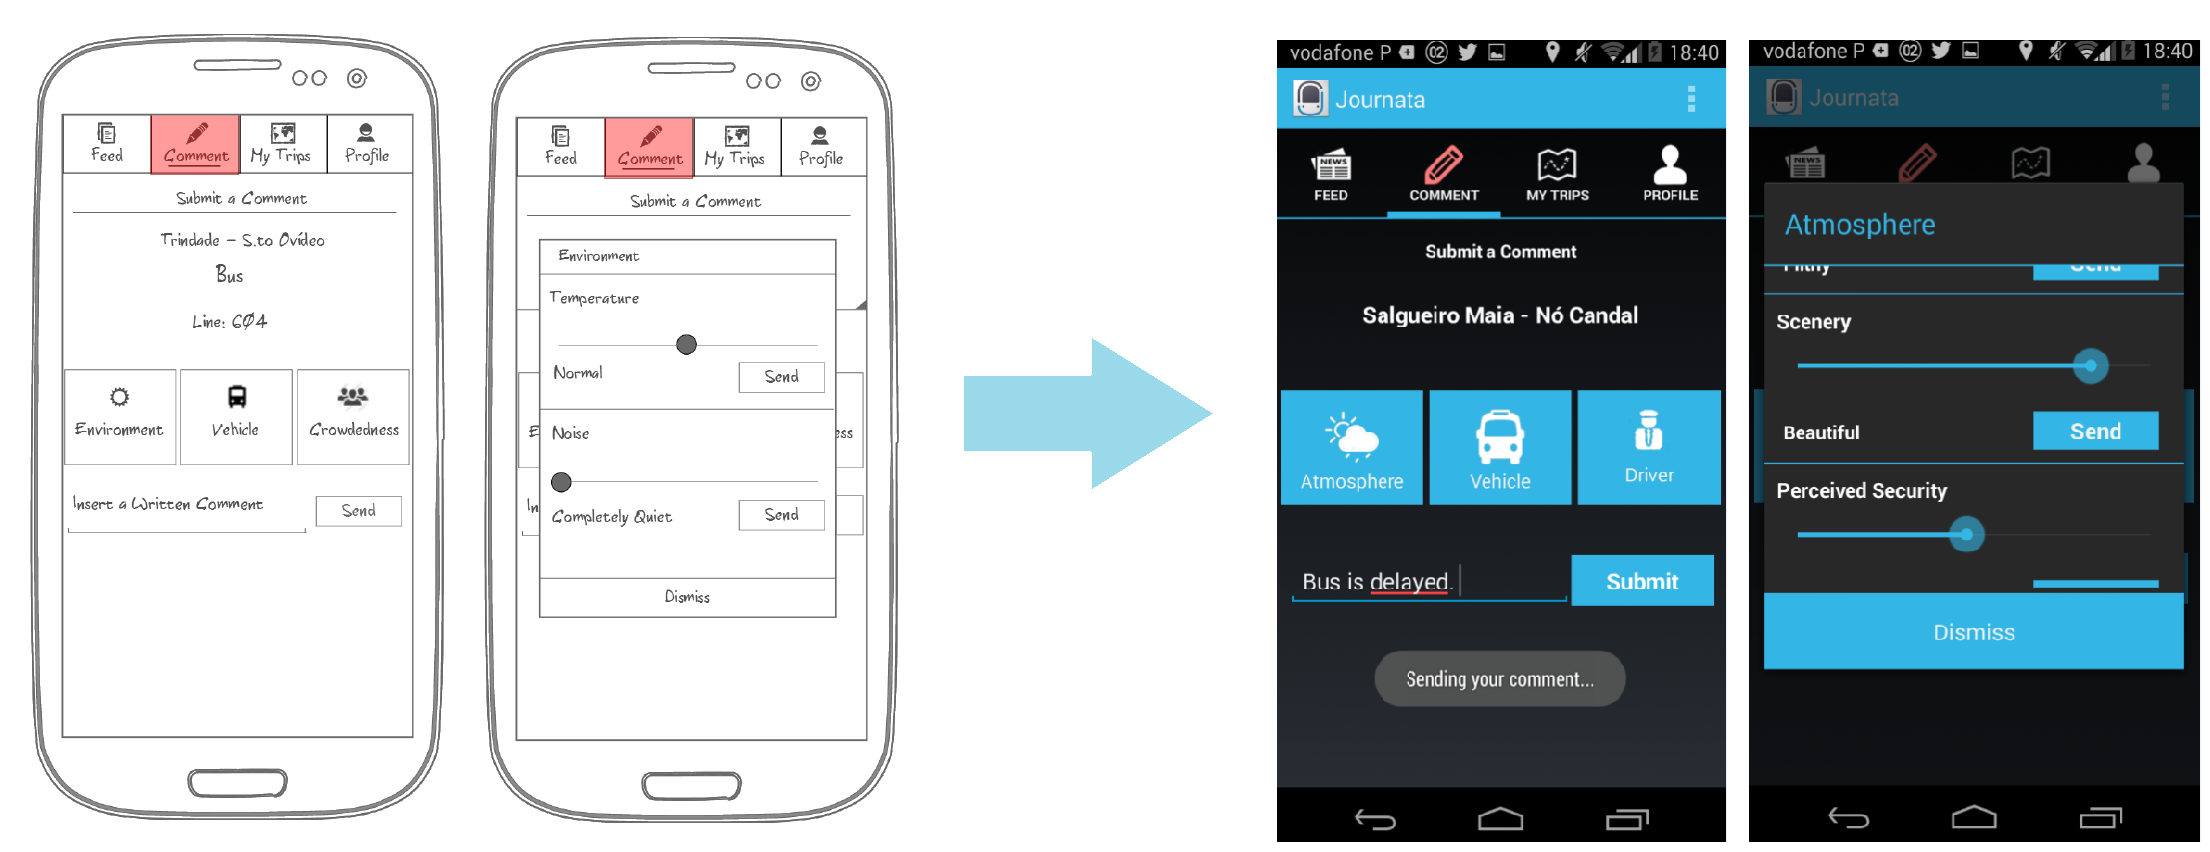
\includegraphics[scale=.15]{artigo.png}}
\caption{Design e implementação da funcionalidade de submissão de comentários.}  
\label{fig:figura}
\end{figure}


\section{Testes e Resultados}

Após a fase de implementação, foi realizada uma sessão de testes junto de \emph{experts} nas áreas de usabilidade e desenvolvimento de aplicações móveis para transportes públicos, que validaram o processo de desenvolvimento da aplicação, reconhecendo a facilidade de uso da aplicação.

Como resultado dessa sessão, foram ainda dadas diversas contribuições e recomendações relativas à interacção presente na aplicação, que deverão ser seguidas e implementadas numa futura iteração da mesma.

Essa sessão possibilitou também alguma discussão relativa a questões que poderão ser exploradas com mais profundidade no futuro, como o novo sistema de pontuações ou a possível agregação de vários comentários num só, e que deverão ser discutidas junto de potenciais utilizadores.

\section{Conclusões}\label{sec:conclui}

Após a realização deste trabalho, conclui-se que a nova iteração da aplicação é um grande passo na direcção correcta, confirmando o grande potencial do projecto. Há ainda, no entanto, muitos aspectos para serem explorados no futuro.

\subsection{Trabalho Futuro}
O desenvolvimento desta aplicação continuará no âmbito de um projecto para desenvolvimento de uma solução de larga escala envolvendo pagamentos móveis nos transportes públicos, com vista à desmaterialização dos títulos de transporte.

Reconhece-se ainda a necessidade de melhorar a arquitectura de dados que serve de suporte à aplicação, de modo a permitir o funcionamento total de algumas das alterações introduzidas no desenvolvimento deste trabalho. A introdução de técnicas de dedução de padrões de viagem dos utilizadores seria também uma mais-valia para a aplicação. 

Discute-se ainda a integração do \textbf{Journata} com algumas redes sociais existentes, e com algumas aplicações relacionadas com transportes públicos numa perspectiva de eliminar o processo de check-in através da sua substituição por um processo de validação automática (via \emph{NFC}, por exemplo).


%%English version: comment first, uncomment second
%\bibliographystyle{unsrt-pt}  % numeric, unsorted refs
%\bibliographystyle{unsrt}  % numeric, unsorted refs
%\bibliography{refs}

\end{multicols}

\end{document}
